%%%%%%%%%%%%%%%%%%%%%%%%%%%%%%%%%%%%%%%%%%%%%%%%%%%%%%%%%%%%%%%%%%%
%                                                                 %
%                            CHAPTER FIVE                         %
%                                                                 %
%%%%%%%%%%%%%%%%%%%%%%%%%%%%%%%%%%%%%%%%%%%%%%%%%%%%%%%%%%%%%%%%%%%

\chapter{MACHINE-READABLE CHANGE LOG}\label{ch:changelog}

\subsection{Produce Change Log}

Change logs were generated for both the Noble Gas data set and the Copper data set.
Following the practices of other change logs, the documents present before and after values for comparison which can be seen in Figure \ref{changelog_zoomed}.
\begin{figure}
	\centering
	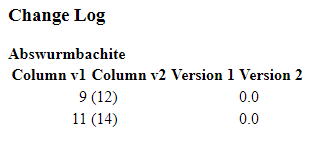
\includegraphics[scale=0.80]{figures/Changelog-zoomed.png}
	\caption{Abswurmbachite entry in the Copper Dataset Change Log}
	\label{changelog_zoomed}
\end{figure}
The partial snapshot of the change log shows that column numbers in the Copper data set also accompany the values to identify the data's location in the spreadsheet.
Very little natural language is used in this change log to regularize the format and improve compatibility with RDFa.
The change logs follow a common format with three sections: Additions, Invalidations, and then Modifications.
The sections may be further grouped by column or row additions.
The division means that changes are not published into the change log as they are found, but instead organized and grouped beforehand.

Employing RDFa means that the document must be written using HTML formatting.
Listing \ref{rdfa_list} shows the text necessary to layout the first four lines of Figure \ref{changelog_zoomed}.
While the content only shows four lines, the underlying markup takes up three and a half times as many lines.
Line 2 states that all following resources will be \textbf{attributes} of Version 1.
Line 3 defines such an \textbf{attribute}.
Lines 5 through 8 define the changes Abswurmbachite undergoes.
Because RDFa allows the statements to be embedded within the content, the triples can appear along with the text they describe.
Lines 11 and 12 define complete triples which do not appear in the visible document.
The lines complete the graph, but must be included in spans because RDFa only allows a single triple within each tag.
Modifying the tags' order so that the spans are unnecessary would cause the visible content to appear in an un-logical order, rendering the document machine-readable but not human-readable.

\begin{lstlisting}[language=HTML, caption=Abswurmbachite RDFa, label=rdfa_list]
<h3>Change Log</h3>
<div about="Version1" rel="vo:hasAttribute">
<div resource="v2:Abswurmbachite" typeof="vo:Attribute">
<span style="font-weight:bold" property="http://www.w3.org/2000/01/rdf-schema#label">Abswurmbachite</span>
<table rel="vo:Undergoes">
<tr  about="ChangeAbswurmbachite12" typeof="vo:Change">
<td align="right" rev="vo:Undergoes" resource="v1:AttributeAbswurmbachite12v1" typeof="vo:Attribute"> 9</td>
<td property="vo:resultsIn" resource="v2:AttributeAbswurmbachite12v2" typeof="vo:Attribute">(12)</td>
<td>          </td>
<td>       0.0</td>
<span about="Version1" property="vo:hasAttribute" resource="v1:AttributeAbswurmbachite12v1"></span>
<span about="Version2" property="vo:hasAttribute" resource="v2:AttributeAbswurmbachite12v2"></span>
</tr>
</table></div></div><br>
\end{lstlisting}

After encountering the limitations of using RDFa to include the versioning graph into the change log, JSON-LD was used.
The new format does not rely on the structure of visible content to determine the syntax triples use to be included in the change log.
Listing \ref{json_list} provides the alternative encoding of the Abswurmbachite entry from RDFa.
The entry is significantly longer, almost three times longer than the RDFa entry and ten times longer than the original visible content.
Instead of including all the data in the beginning or end of the document, each change block is separated into the particular \textit{div} section for that change.
This choice allows consumers to extract pertinent change information without needing to ingest the entire versioning graph.

\begin{lstlisting}[language=HTML, caption=Abswurmbachite JSON-LD, label=json_list]
<h3>Change Log</h3>
<div about="v1:Abswurmbachite">
<span style="font-weight:bold" property="http://www.w3.org/2000/01/rdf-schema#label">Abswurmbachite</span>
<table>
<tr  id="ModifyChangeAbswurmbachite12">
<td align="right"> 9</td>
<td >(12)</td>
<td>          </td>
<td>       0.0</td>
<script type="application/ld+json">
[
{
"@context": "https://orion.tw.rpi.edu/~blee/provdist/GCMD/VO.jsonld", 
"@id": "http://CUdb.com/v1/AttributeAbswurmbachite9", 
"@reverse": {
"hasAttribute": "Version1"
}, 
"@type": "vo:Attribute", 
"label": "Primary", 
"undergoes": "http://orion.tw.rpi.edu/~blee/provdist/CU/DTDI/CUjsonlog.html#ModifyChangeAbswurmbachite12"
}, 
{
"@context": "https://orion.tw.rpi.edu/~blee/provdist/GCMD/VO.jsonld", 
"@id": "http://orion.tw.rpi.edu/~blee/provdist/CU/DTDI/CUjsonlog.html#ModifyChangeAbswurmbachite12", 
"@type": "vo:ModifyChange", 
"resultsIn": "http://CUdb.com/v2/AttributeAbswurmbachite12"
}, 
{
"@context": "https://orion.tw.rpi.edu/~blee/provdist/GCMD/VO.jsonld", 
"@id": "http://CUdb.com/v2/AttributeAbswurmbachite12", 
"@reverse": {
"hasAttribute": "Version2"
}, 
"@type": "vo:Attribute", 
"label": "Primary"
}
]
</script>
</tr>
</table></div><br>
\end{lstlisting}

The encoded change logs struggle with intense document size.
The Copper Minerals data set encoded in RDFa is 1.7 MB and JSON-LD is 3.3 MB.
In the Noble Gas data set, the RDFa and JSON-LD change log sizes are 59 and 60 MB, respectively.
The Noble Gas change logs often do not load in a browser.

\begin{table}[b]
	\caption{Sizes of change log encodings.}
	\label{changelog_table}
	\centering
	\begin{tabular}{|c|c|c|c|}
		\hline
		Dataset & No Encoding (MB) & RDFa (MB) & JSON-LD (MB) \\
		\hline
		Copper Minerals & 0.137 & 1.7 & 3.4 \\
		Noble Gas & 5.4 & 59 & 124 \\
		\hline
	\end{tabular}
\end{table}

